

\documentclass[3p,12pt ]{elsarticle}

\makeatletter
\def\ps@pprintTitle{%
 \let\@oddhead\@empty
 \let\@evenhead\@empty
 \let\@oddfoot\@empty
 \let\@evenfoot\@empty
}
\makeatother


%% Use the option review to obtain double line spacing
%% \documentclass[preprint,review,12pt]{elsarticle}

%% Use the options 1p,twocolumn; 3p; 3p,twocolumn; 5p; or 5p,twocolumn
%% for a journal layout:
%% \documentclass[final,1p,times]{elsarticle}
%% \documentclass[final,1p,times,twocolumn]{elsarticle}
%% \documentclass[final,3p,times]{elsarticle}
%% \documentclass[final,3p,times,twocolumn]{elsarticle}
%% \documentclass[final,5p,times]{elsarticle}
%% \documentclass[final,5p,times,twocolumn]{elsarticle}

%% For including figures, graphicx.sty has been loaded in
%% elsarticle.cls. If you prefer to use the old commands
%% please give \usepackage{epsfig}
%% The amssymb package provides various useful mathematical symbols



\usepackage{natbib}
 \bibpunct[, ]{(}{)}{,}{a}{}{,}%
 \def\bibfont{\small}%
 \def\bibsep{\smallskipamount}%
 \def\bibhang{24pt}%
 \def\newblock{\ }%
 \def\BIBand{and}%

\usepackage{lipsum} 
\usepackage{amssymb}
\usepackage{amsmath}
\usepackage{booktabs}
\usepackage{longtable}
\usepackage{array}
\usepackage{multirow}
\usepackage{wrapfig}
\usepackage{float}
\usepackage{colortbl}
\usepackage{pdflscape}
\usepackage{tabu}
\usepackage{threeparttable}
\usepackage{threeparttablex}
\usepackage[normalem]{ulem}
\usepackage{makecell}
\usepackage{xcolor}

\usepackage{booktabs}   % for top/mid/bottomrule
\usepackage{dcolumn}    % for D column alignment
\usepackage{caption}    % optional, for better caption formatting
\usepackage{amsmath}    % optional, for symbols like chi²

%\usepackage[nomarkers]{endfloat}
\usepackage{setspace}
\usepackage{graphicx}
\usepackage{float}
\usepackage{rotating}
\usepackage{hyperref}
\hypersetup{
  colorlinks=true,
  linkcolor=blue}
\usepackage{caption}
\captionsetup{font=normalsize}

%% The amsthm package provides extended theorem environments
%% \usepackage{amsthm}

%% The lineno packages adds line numbers. Start line numbering with
%% \begin{linenumbers}, end it with \end{linenumbers}. Or switch it on
%% for the whole article with \linenumbers.
%% \usepackage{lineno}

\journal{Housing studies}

\begin{document}

\begin{frontmatter}

%% Title, authors and addresses

%% use the tnoteref command within \title for footnotes;
%% use the tnotetext command for theassociated footnote;
%% use the fnref command within \author or \address for footnotes;
%% use the fntext command for theassociated footnote;
%% use the corref command within \author for corresponding author footnotes;
%% use the cortext command for theassociated footnote;
%% use the ead command for the email address,
%% and the form \ead[url] for the home page:
%% \title{Title\tnoteref{label1}}
%% \tnotetext[label1]{}
%% \author{Name\corref{cor1}\fnref{label2}}
%% \ead{email address}
%% \ead[url]{home page}
%% \fntext[label2]{}
%% \cortext[cor1]{}
%% \affiliation{organization={},
%%             addressline={},
%%             city={},
%%             postcode={},
%%             state={},
%%             country={}}
%% \fntext[label3]{}

\title{The value of location: what matters most for older home owners in Sweden?}

%% use optional labels to link authors explicitly to addresses:
%% \author[label1,label2]{}
%% \affiliation[label1]{organization={},
%%             addressline={},
%%             city={},
%%             postcode={},
%%             state={},
%%             country={}}
%%
%% \affiliation[label2]{organization={},
%%             addressline={},
%%             city={},
%%             postcode={},
%%             state={},
%%             country={}}

\author[1]{Nick Christie}
\ead{nick.christie@med.lu.se}

\author[1]{Susanne Iwarsson}
\ead{susanne.iwarsson@med.lu.se}

\author[1]{Magnus Zingmark}
\ead{magnus.zingmark@med.lu.se}

%\author[1]{Maya Ky\'eln}
%\ead{maya.kyeln@med.lu.se}

\author[1]{Bj\"orn Slaug}
\ead{bjorn.slaug@med.lu.se}

\author[2]{Jonas Bj\"ork}
\ead{jonas.bjork@med.lu.se}



%\author[1]{Steven M Schmidt}
%\ead{steven.schmidt@med.lu.se}















 \affiliation[1]{organization={Department of Health Sciences, Lund University}, 
                 addressline={P.O. Box 7080},
                 postcode={22100}, 
                 city={Lund}, 
                 country={Sweden}}
                 
 \affiliation[2]{organization={Division of Occupational and Environmental Medicine, Lund University}, 
                 addressline={Scheelevägen 2},
                 postcode={22363}, 
                 city={Lund}, 
                 country={Sweden}}
                 
                 
\begin{abstract}

This study examines variation in housing attribute preferences among older adults in Sweden using a discrete choice experiment conducted with a stratified sample of older individuals registered with housing relocation services. The experimental design incorporates key locational attributes including proximity to services, access to public transportation, availability of green space, and presence dedicated parking facilities. These attributes are framed using percentage-based trade-offs to estimate marginal willingness to pay for each feature. Socio-demographic factors such as age and gender are included to identify systematic differences in preferences. The results reveal substantial heterogeneity. Individuals in the oldest age groups express significantly higher willingness to pay for several attributes, with some values reaching up to three times those of younger respondents. Differences between men and women are also observed. The findings provide evidence-based estimates that support policy development and housing planning aimed at facilitating ageing in place and improving the design of environments that accommodate diverse needs in later life.
\end{abstract}


%\begin{keyword}
%
%Ageing \sep Housing \sep Health \sep Relocation
%%% keywords here, in the form: keyword \sep keyword
%
%%% PACS codes here, in the form: \PACS code \sep code
%
%%% MSC codes here, in the form: \MSC code \sep code
%%% or \MSC[2008] code \sep code (2000 is the default)
%
%\end{keyword}
\end{frontmatter}

%% \linenumbers

\newpage



\section{Introduction}

As populations age and the expansion of housing associated with boundless population growth maintains pace,
understanding the locational preferences of the ageing demographic becomes increasingly vital for future societies.
In Sweden, the majority of senior citizens are living in their own homes with 94\% of the population aged 65+ living in ordinary housing \citep{jennbertDevelopmentsElderlyPolicy2009}.
As this population segment grows,
appropriate housing options are essential to provide viable options for an ageing society in need of housing.
Striking the right balance between housing attributes is a complex decision-making process in the search for new accommodation,
with the considerations of the older populations even more relevant today.

This study employs a discrete choice experiment (DCE) to delve into the critical factors influencing the housing choices of older home owners in Sweden wishing to relocate to an apartment setting. Our research uses a diverse sample of older home owners, presenting them with hypothetical scenarios that vary in locational attributes, including proximity to healthcare facilities, access to public transportation, green spaces, social amenities, and natural surroundings.
Leverage the identification of key housing attributes from the nation-wide RELOC-AGE study,
we are able to take a closer look at the factors which matter most for older home owners wishing to relocates.
In analysing their responses, we are able to not only elicit preferences and estimate the relative importance of these attributes,
but also to estimate their willingness to pay for these attributes.

Among these attributes, two factors stand out as paramount: access to public transportation and proximity to green spaces.
These findings provide valuable insights for rural planners, policy-makers, and healthcare providers, offering guidance on creating age-friendly environments that cater to the unique needs and desires of older home owners while fostering resilient communities.
In this context, understanding the interplay between these key factors is essential for optimizing the rural living experience for the older population, ensuring their well-being and continued contribution to the vitality of future societies.

\section{Sample and Method}

\subsection{Sample}

This paper utilizes follow-up data derived from the prospective RELOC-AGE study,
which is a longitudinal two-tiered mixed-method cohort investigation conducted in Sweden.
The study was registered under the identifier NCT04765696 on ClinicalTrials.gov (U.S. National Library of Medicine, 2021).
\footnote{For comprehensive insights into the study's procedures,
please refer to the study protocol  \cite{zingmarkExploringAssociationsHousing2021}}
The initial data collection took place from March to December 2021, with one-year follow-up surveys conducted in 2022, and the DCE experiment conducted in 2024.
A geographical diverse sample of home owners aged 55 and above was recruited for this study across Sweden (see Figure \ref{fig:map})

The primary objective of the prospective RELOC-AGE study was to explore the long-term dynamics associated with housing choices, relocation, and active and healthy ageing, focusing on individuals in the early stages of the ageing process.
In Sweden, approximately 4-5\% of individuals aged 60-84 years relocate each year (Statistics Sweden, 2020).
Accordingly, the study aimed to recruit a diverse and information-rich sample, including individuals who might have a higher likelihood of relocating.
Eligible participants were individuals aged 55 or older, residing in Sweden, and actively registered for relocation with one of three housing companies.
\begin{wrapfigure}[25]{r}{0.2\textwidth}
\centering
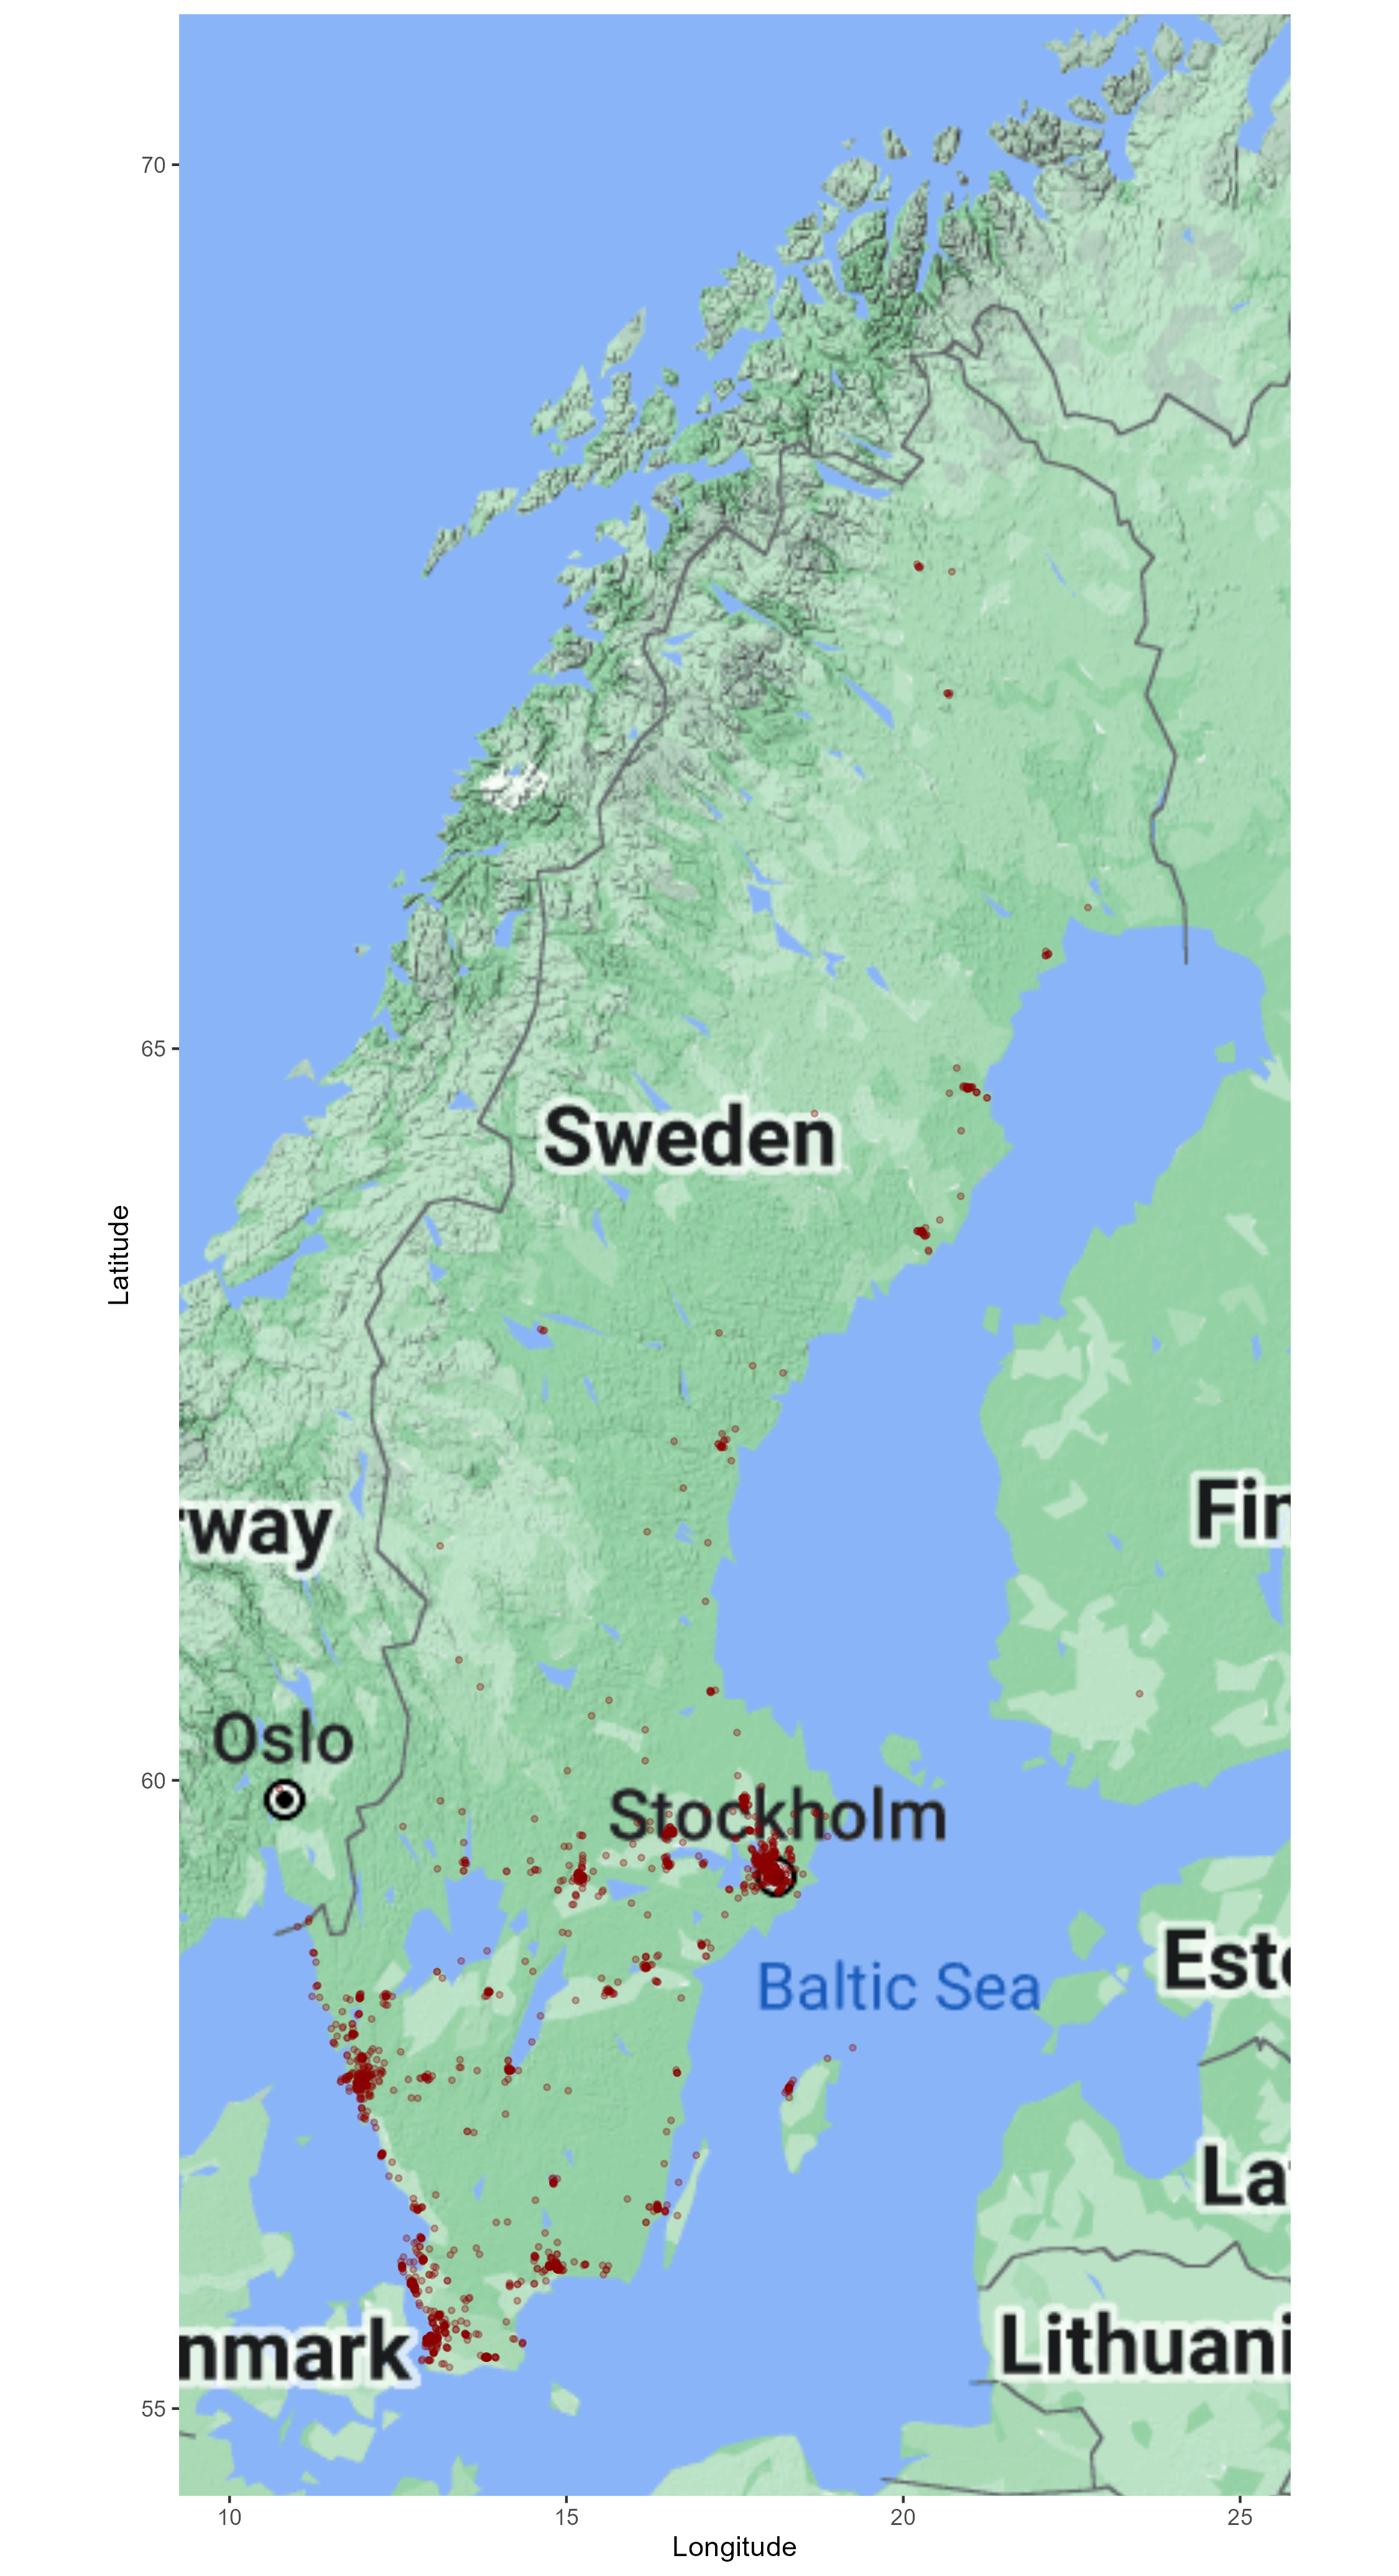
\includegraphics[scale=0.25]{figures/survey_location.png}
\caption{Country distribution of respondents \label{fig:map}}
\end{wrapfigure}
These housing companies included two local public housing providers and a national provider of tenant-owned dwellings, thereby representing various types of multi-family housing typically appealing to individuals from different socio-economic backgrounds. 

During the recruitment phase in 2021, an invitation letter inviting participation was sent by postal mail to 8,583 potential participants registered for relocation with the aforementioned housing companies.
The letter provided details about the project, its procedures, data handling in accordance with existing regulations, and emphasized the voluntary nature of participation.
A reminder was sent to those who had expressed interest in the study. Ultimately, 1,964 individuals agreed to participate and responded to the baseline survey. Following verification with the Swedish Tax Agency to identify any deceased participants, an invitation letter for the one-year follow-up was sent by postal mail to 1,952 participants on two occasions: in May (973 recipients) and September (979 recipients). In total, 1,509 participants responded to the second survey, resulting in a response rate of 77.3\%.




The choice experiment was administered in January 2024,
where 1,297 of the 1,952 original respondents agreed to participate in the study.
Respondents who had already relocated and those who did not fully complete the survey questions were excluded, leading to a final sample size of 978 individuals.
Table \ref{tab:des} presents the results.
Among the sample, 55\% were female, 46\% were male, and the majority (64\%) reported being married or cohabiting with a partner. Additionally, 73\% of respondents fell within the age range of 54-74, and the majority rated their health as either good (34\%) or very good (33\%).

\begin{table}


%\begin{wraptable}{r}{0.4\textwidth} 
\begin{table}[h]
\centering
\caption{Descriptive statistics}
\label{tab:desc}
\begin{threeparttable}
\begin{tabular}{lccc}
\scriptsize
\toprule
 & \textbf{Owner (N=790)} & \textbf{Renter (N=167)} & \textbf{Overall (N=957)} \\
\midrule
\textbf{Sex} \\
\hspace{1em}Female & 419 (53.0\%) & 110 (65.9\%) & 529 (55.3\%) \\
\hspace{1em}Male & 371 (47.0\%) & 57 (34.1\%) & 428 (44.7\%) \\

\textbf{Age group} \\
\hspace{1em}55--64 & 154 (19.5\%) & 38 (22.8\%) & 192 (20.1\%) \\
\hspace{1em}65--74 & 344 (43.5\%) & 72 (43.1\%) & 416 (43.5\%) \\
\hspace{1em}75+ & 292 (37.0\%) & 57 (34.1\%) & 349 (36.5\%) \\

\textbf{Civil status} \\
\hspace{1em}Not partnered & 287 (36.3\%) & 90 (53.9\%) & 377 (39.4\%) \\
\hspace{1em}Partnered & 503 (63.7\%) & 77 (46.1\%) & 580 (60.6\%) \\

\textbf{Retired} \\
\hspace{1em}Yes & 612 (77.5\%) & 126 (75.4\%) & 738 (77.1\%) \\
\hspace{1em}No & 174 (22.0\%) & 41 (24.6\%) & 215 (22.5\%) \\
\hspace{1em}Missing & 4 (0.5\%) & 0 (0.0\%) & 4 (0.4\%) \\

\textbf{Current housing type} \\
\hspace{1em}Apartment/Condo & 447 (56.6\%) & 153 (91.6\%) & 600 (62.7\%) \\
\hspace{1em}House & 341 (43.2\%) & 13 (7.8\%) & 354 (37.0\%) \\
\hspace{1em}Missing & 2 (0.3\%) & 1 (0.6\%) & 3 (0.3\%) \\

\textbf{Current housing location} \\
\hspace{1em}City/town & 478 (60.5\%) & 117 (70.1\%) & 595 (62.2\%) \\
\hspace{1em}Urban area & 221 (28.0\%) & 41 (24.6\%) & 262 (27.4\%) \\
\hspace{1em}Countryside & 81 (10.3\%) & 6 (3.6\%) & 87 (9.1\%) \\
\hspace{1em}Missing & 10 (1.3\%) & 3 (1.8\%) & 13 (1.4\%) \\

\textbf{Monthly household income} \\
\hspace{1em}Mean (SD) & 48700 (34700) & 37700 (27900) & 46700 (33900) \\
\hspace{1em}Median [Min, Max] & 44300 [0, 220000] & 35000 [0, 153000] & 40500 [0, 220000] \\
\hspace{1em}Missing & 6 (0.8\%) & 0 (0.0\%) & 6 (0.6\%) \\

\textbf{Planned housing costs} \\
\hspace{1em}Mean (SD) & 10400 (4060) & 10500 (5570) & 10500 (4370) \\
\hspace{1em}Median [Min, Max] & 10000 [3000, 40000] & 9000 [3000, 60000] & 10000 [3000, 60000] \\
\hspace{1em}Missing & 95 (12.0\%) & 15 (9.0\%) & 110 (11.5\%) \\
\bottomrule
\end{tabular}
\end{threeparttable}
\end{table}

%\end{wraptable}

\end{table}

\clearpage

\subsection{Section on motivation of stratification}

This section motivates the reasoning to estimate the tests along different strata.
For example,
if we were interested in examining the willingness to pay across education levels we could develop that here while also including some figures to show the representativeness in our sample such as Figure \ref{fig:edu}.


\begin{figure}[H]

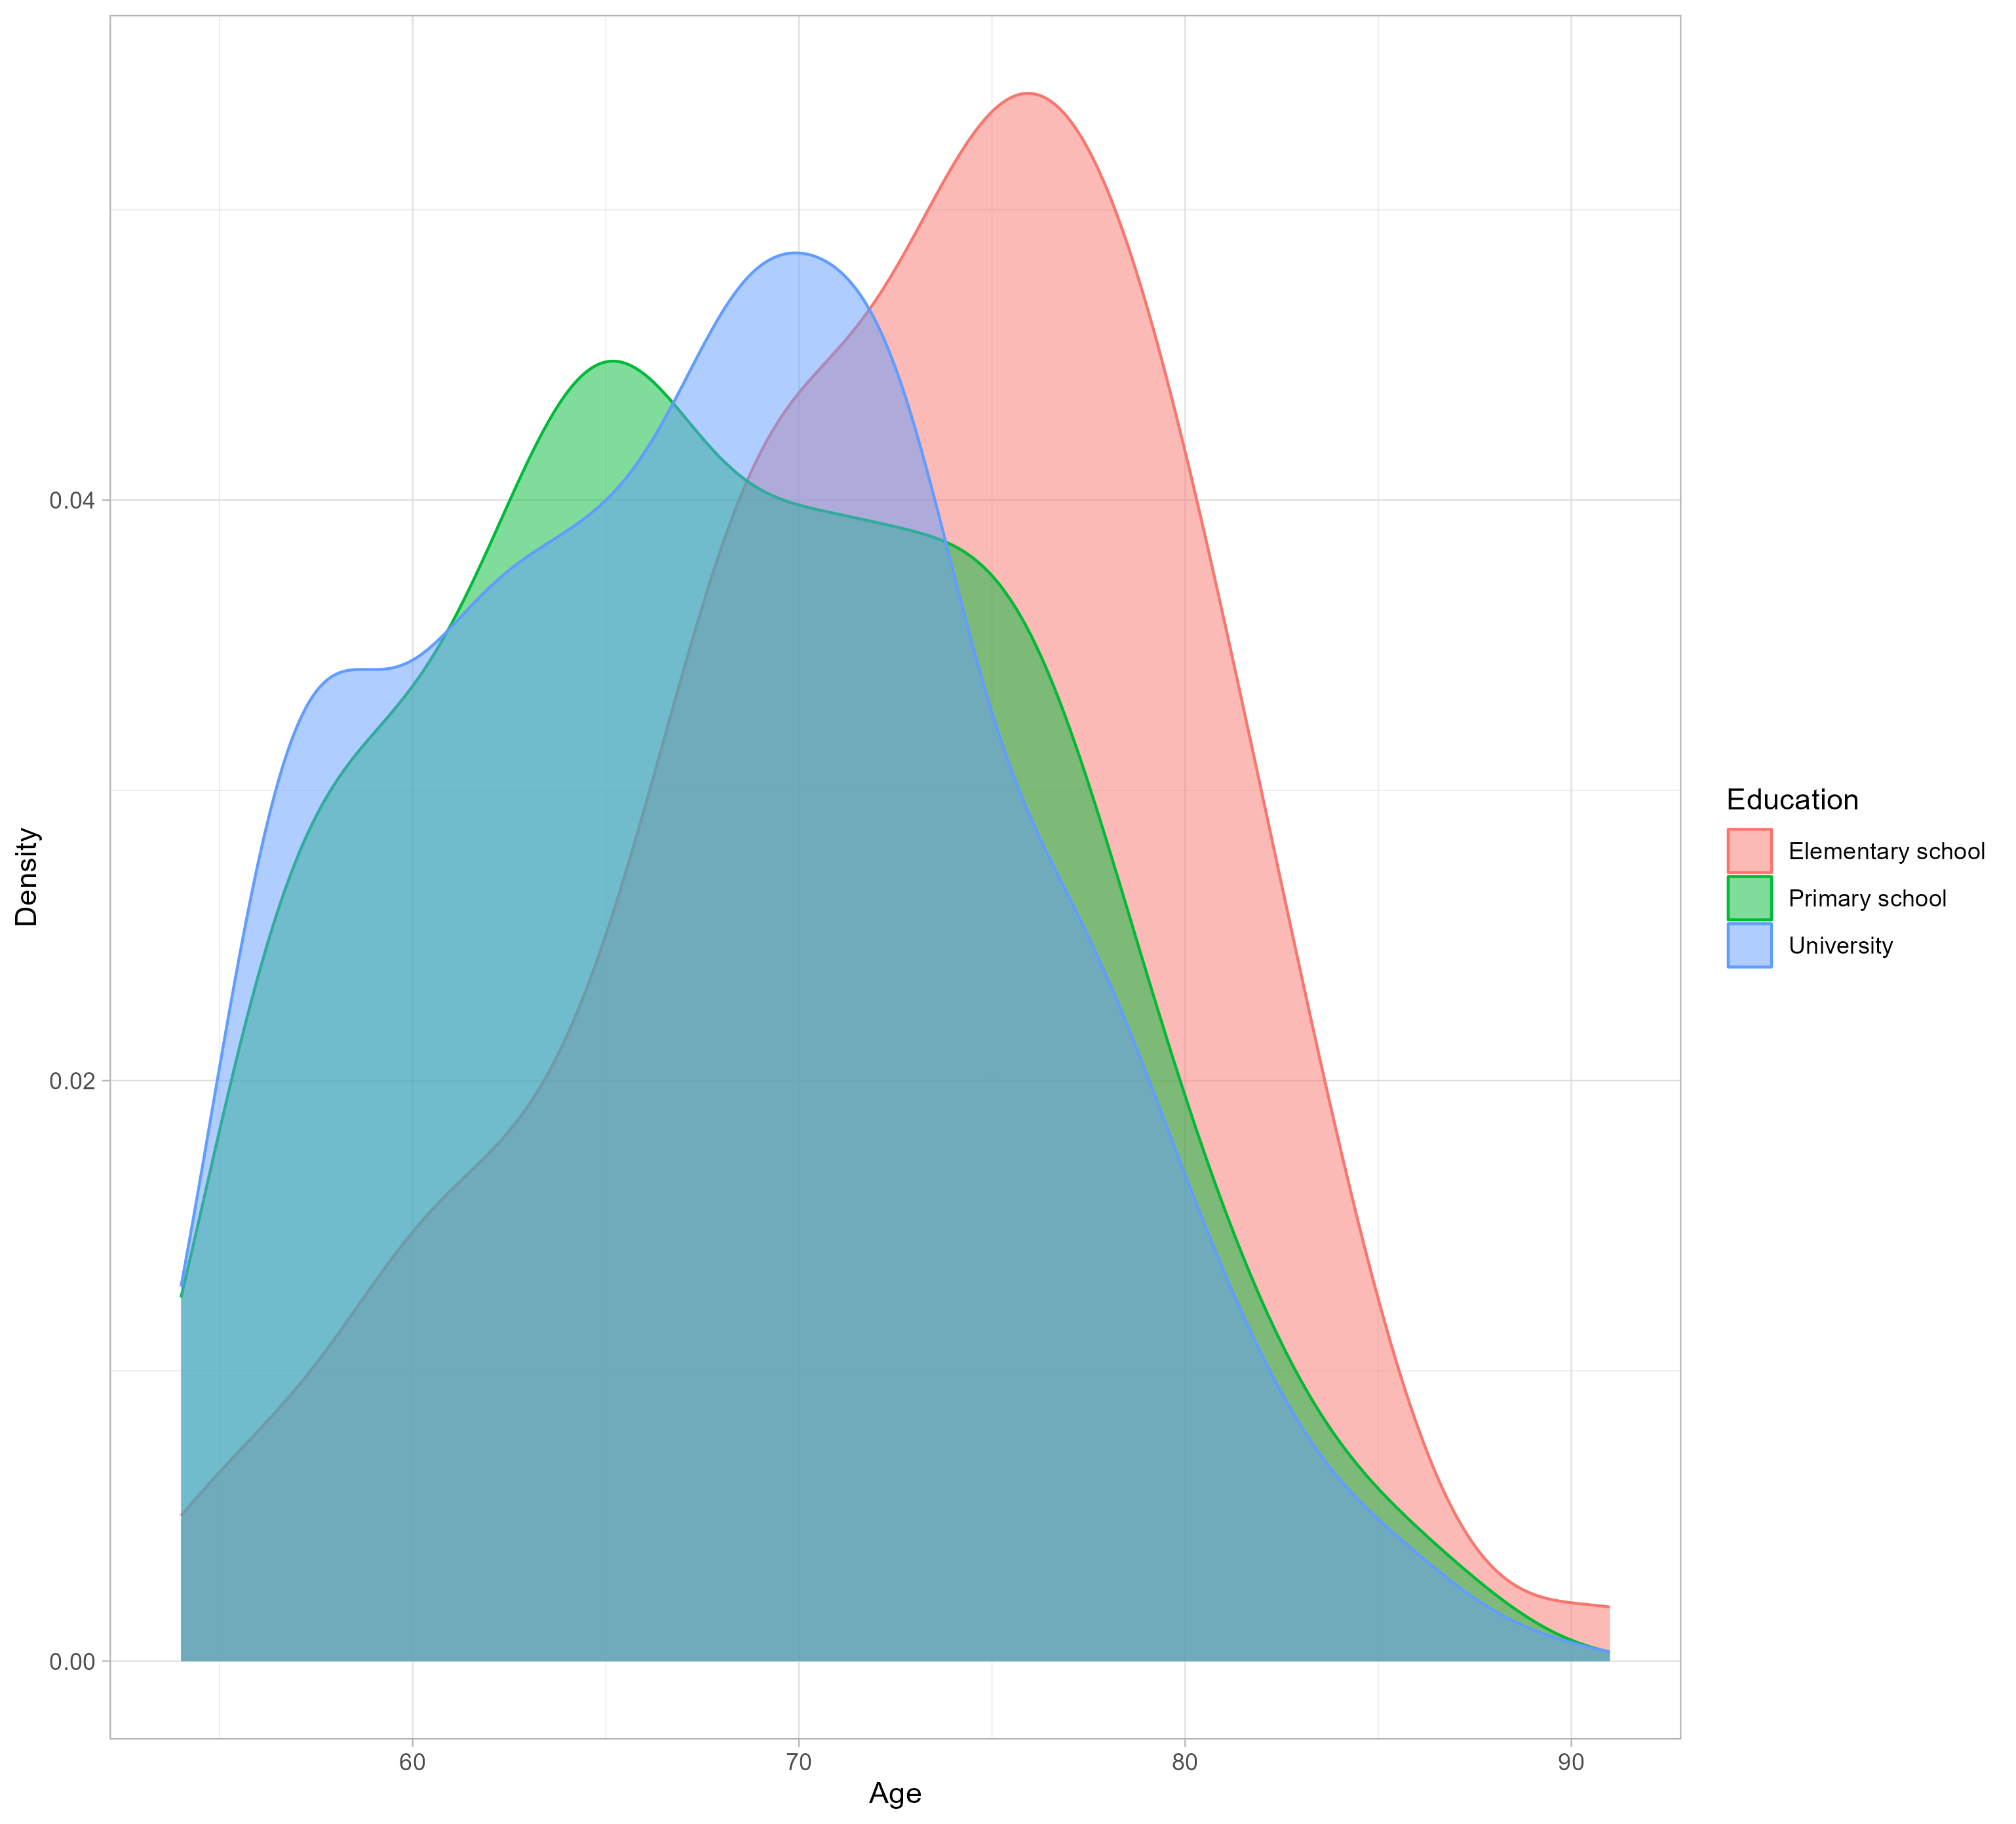
\includegraphics[width=\textwidth]{figures/edu_den.png}
\vspace{1mm}
\footnotesize \textit{Note:} Figure shows density plot of age stratified by educational level for survey respondents in Sweden.
\caption{Age distribution across education \label{fig:edu}}
\end{figure}



\newpage

\subsection{Experimental design}

This study utilizes a discrete choice experiment (DCE) to investigate the locational preferences of older home owners wishing to relocate to apartments in Sweden.
A DCE is a quantitative research method that presents respondents with a series of hypothetical scenarios, each with varying attributes, to elicit preferences and estimate the relative importance of these attributes in decision-making \citep{lancsarConductingDiscreteChoice2008}.
The utility that an individual assigns to a particular choice alternative is estimated using a conditional logit model based on random utility theory.
The utility of an alternative is represented as:

\begin{equation}
U_{ij} = V_{ij} + \varepsilon_{ij}
\end{equation}

\noindent where $U_{ij}$ is the total utility that respondent \textit{i} associates with choice alternative \textit{j} and $V_{ij}$ is the systematic utility, which is a function of the attributes of the alternative and the preferences of the respondent.
$\varepsilon_{ij}$ is the random error term, representing unobserved factors and individual-specific preferences.
The systematic utility, \( V_{ij} \), is modelled as a linear function of attribute levels:

\begin{equation}
V_{ij} = \beta_1 X_{ij1} + \beta_2 X_{ij2} + \ldots + \beta_k X_{ijk}
\end{equation}

\noindent where $\beta_1$, $\beta_2$, $\ldots$, $\beta_k$  are the coefficients representing the part-worth utilities of the attribute levels and $X_{ij1}$, $X_{ij2}$, $\ldots$, $X_{ijk}$ are the levels of the attributes for choice alternative \textit{j} in scenario \textit{i}.

\vspace{2mm}

\noindent The probability that respondent \( i \) chooses alternative \( j \) from a set of alternatives is modeled using the choice probability as follows:

\begin{equation}
P_{ij} = \frac{e^{V_{ij}}}{\sum_{l=1}^{J} e^{V_{il}}}
\end{equation}

\noindent where $P_{ij}$  is the probability that respondent \textit{i} chooses alternative \textit{j}.
\textit{J} is the total number of alternatives in the choice set.
To estimate the coefficients (\( \beta \) values) in the systematic utility equation, maximum likelihood estimation is used.
The likelihood function for the conditional logit model is maximized to find the best-fitting coefficients that maximize the probability of observing the actual choices made by respondents given the attributes of the alternatives.

The estimated coefficients (\( \hat{\beta} \)) are used to further calculate willingness to pay and the relative importance of each attribute highlighting the trade-offs respondents are willing to make between attribute levels when choosing among alternatives.

\section{Method -- }

We constructed an efficient fractional factorial design to minimize the asymptotic variance of the parameters, subject to level balance and minimal overlap constraints. The design was blocked into \textit{<B>} versions so that each respondent faced \textit{<T>} choice sets with two alternatives per set \textit{<plus opt out, if used>}. Attribute level balance and dominance checks were performed during piloting. A brief training screen with an example task was included before the main experiment.

\subsection{Random utility framework}
Let $i$ index individuals, $t = 1,\dots,T_i$ index choice tasks, and $j \in \{1,2\}$ index alternatives \textit{<and $j=0$ for the opt out if included>}. Utility is
\begin{equation}
U_{ijt} = \alpha_j + \mathbf{x}_{ijt}' \boldsymbol{\beta}_i + \beta_{p,i} \, \text{PctCost}_{ijt} + \varepsilon_{ijt},
\end{equation}
where $\mathbf{x}_{ijt}$ is the vector of nonprice attributes, $\text{PctCost}_{ijt}$ is the percentage change in housing cost, and $\varepsilon_{ijt}$ is i.i.d.\ Type I extreme value. The alternative specific constants $\alpha_j$ capture any average preference for each alternative relative to the base. Following \citet{Caplan2021}, we estimate models in preference space and recover willingness to pay measures by ratio to the cost coefficient.

\subsection{Econometric specification and estimation}
We estimate a mixed logit model to allow for unobserved preference heterogeneity:
\begin{equation}
\boldsymbol{\beta}_i = \boldsymbol{\beta} + \mathbf{\Sigma}^{1/2} \mathbf{\eta}_i, \quad \mathbf{\eta}_i \sim \mathcal{N}(\mathbf{0}, \mathbf{I}),
\end{equation}
with $\beta_{p,i}$ either fixed or random with a sign constraint \textit{<state your choice>}. The panel structure of repeated choices per individual is accommodated by integrating the likelihood over the distribution of random coefficients:
\begin{equation}
L_i = \int \prod_{t=1}^{T_i} \frac{\exp\left( V_{i y_{it} t} \right)}{\sum_{j} \exp\left( V_{ijt} \right)} \, f(\boldsymbol{\beta}_i, \beta_{p,i} \mid \boldsymbol{\theta}) \, d\boldsymbol{\beta}_i \, d\beta_{p,i},
\end{equation}
where $V_{ijt} = \alpha_j + \mathbf{x}_{ijt}' \boldsymbol{\beta}_i + \beta_{p,i} \, \text{PctCost}_{ijt}$. Parameters $\boldsymbol{\theta}$ are estimated by simulated maximum likelihood using \textit{<number>} quasi Monte Carlo draws (Halton or Sobol) and clustering standard errors at the individual level. We also report conditional logit estimates as a baseline.

To account for observed heterogeneity, we include interactions between attributes and socio demographic covariates:
\begin{equation}
\mathbf{x}_{ijt}' \boldsymbol{\beta}_i \; \leftarrow \; \mathbf{x}_{ijt}' \boldsymbol{\beta}_i \;+\; \left( \mathbf{x}_{ijt} \otimes \mathbf{z}_i \right)'\boldsymbol{\gamma},
\end{equation}
where $\mathbf{z}_i$ includes age group, gender, and other controls.

\subsection{Willingness to pay}
Marginal willingness to pay for attribute $k$ is computed as the ratio of the attribute coefficient to the cost coefficient:
\begin{equation}
\text{MWTP}_{k,i} \;=\; - \frac{\beta_{k,i}}{\beta_{p,i}}.
\end{equation}
We report mean and percentile summaries of the implied MWTP distribution using the simulated draws of $\beta_{k,i}$ and $\beta_{p,i}$, along with delta method or simulation based standard errors. Because the cost attribute is specified as a percentage change, we convert MWTP to monetary terms by scaling with each respondent's reported or imputed baseline housing cost, consistent with \citet{Caplan2021}.


\section{Attributes}

The choice of attributes and associated levels in our study are a combination of important factors identified from the RELOC-AGE follow-up study and attributes found in the housing literature.
Following standard practice,
we select levels that allow for interpretability and viability of our willingness to pay estimates while holding certain attributes constant to make meaningful comparisons \citep{hensherAppliedChoiceAnalysis2015}.
The number of attributes is limited to 5 in order to minimize the cognitive burden of the DCE \citep{manghamHowNotDesigning2009,deshazoDesigningChoiceSets2002}
\footnote{\cite{himmlerWhatWorksBetter2021} highlights increased age would tend to exacerbated the cognitive burden of a discrete choice experiment, suggesting complex designs would lead to unreliable results.}.


Table \ref{tab:atts} shows the attributes selected and their associated levels.
The variable \textit{greenclose} is defined as the distance in kilometres to green areas including parks, forests, hiking areas, and open spaces.
The shortest distance of 5km represents the base level category in our analysis.
Similarly,
\textit{shopsclose} represents the distance to shopping amenities such as grocery stores, malls, boutiques, and shopping centres.
\textit{Price} represents the percentage change in price the respondents for each alternative,
where monthly housing costs are known a priori from the initial questions on the survey.
Further describe and motivate the attributes...

\begin{table}[H]
\scriptsize
\caption{Attributes and descriptions \label{tab:atts}}
\centering
\begin{tabular}[top]{>{\raggedright\arraybackslash}p{15em}l}
\toprule
Attribute & Description and levels\\
\midrule
Distance to green area & \makecell[l]{1 = within 500m \\ 2 = within 10km \\ 3 = within 15km}\\
\addlinespace
Distance to shops & \makecell[l]{1 = within 500m \\ 2 = within 10km \\ 3 = within 15km}\\
\addlinespace
Distance to public transportation & \makecell[l]{1 = within 300m \\ 2 = within 600 \\ 3 = within 900m}\\
\addlinespace
Parking & \makecell[l]{1 = no reserved parking \\ 2 = reserved parking place \\ 3 = reserved garage place}\\
\addlinespace
Price & \makecell[l]{1 = 20 \% less than planned costs \\ 2 = 10 \% less than planned costs \\ 3 = same as planned cost \\ 4 = 10 \% more than planned costs  \\ 5 = 20 \% more than planned costs}\\
\bottomrule
\end{tabular}
\end{table}


\clearpage

\section{Empirical Results}

This section discusses the results from the baseline tests and continuing to the results from our tests stratified by education.
In interpreting the results,
all else being equal, 
a positive coefficient estimate for a given variable indicates an increase in the utility level for an average person in the sample for in comparison to the particular variable's base level.
To asses the relative importance of the attributes,
the magnitude of the coefficient estimates can be compared.

Table \ref{tab:base_male} presents results from our baseline study where column one refers to the model including only male respondents.



\begin{table}[h]
\caption{Baseline results - Male}
\label{table:base_male}
\begin{center}
\scriptsize
\begin{tabular}{l D{.}{.}{5.5} D{.}{.}{5.5} D{.}{.}{2.5} D{.}{.}{2.5} D{.}{.}{3.2}}
\toprule
 & & \multicolumn{2}{c}{MXL} \\
\cmidrule(lr){3-4}
 & \multicolumn{1}{c}{MNL} & \multicolumn{1}{c}{Mean} & \multicolumn{1}{c}{SD} & \multicolumn{1}{c}{MRS} & \multicolumn{1}{c}{MWTP (SEK/mo)} \\
\midrule
Green space: 5 km (vs 15 km)       & 0.65^{***}  & 1.33^{***}  & -0.25       & 0.23^{***} & 227.78 \\
                                   & (0.07)      & (0.16)      & (0.24)      & (0.03)     &        \\
Green space: 500 m (vs 15 km)      & 1.01^{***}  & 2.05^{***}  & 1.16^{***}  & 0.35^{***} & 351.54 \\
                                   & (0.07)      & (0.20)      & (0.32)      & (0.04)     &        \\
Shops: 5 km (vs 15 km)             & 0.69^{***}  & 1.26^{***}  & 0.32        & 0.22^{***} & 215.57 \\
                                   & (0.08)      & (0.18)      & (0.26)      & (0.04)     &        \\
Shops: 500 m (vs 15 km)            & 1.76^{***}  & 3.45^{***}  & 0.17        & 0.59^{***} & 590.67 \\
                                   & (0.07)      & (0.25)      & (0.30)      & (0.05)     &        \\
Transit stop: 600 m (vs 900 m)     & 0.20^{**}   & 0.32^{*}    & -1.14^{***} & 0.05       & 54.05  \\
                                   & (0.08)      & (0.16)      & (0.23)      & (0.03)     &        \\
Transit stop: 300 m (vs 900 m)     & 0.41^{***}  & 0.85^{***}  & 0.21        & 0.15^{***} & 145.00 \\
                                   & (0.07)      & (0.16)      & (0.20)      & (0.03)     &        \\
Parking: reserved garage (vs none) & 1.71^{***}  & 3.65^{***}  & -1.54^{***} & 0.62^{***} & 624.07 \\
                                   & (0.08)      & (0.29)      & (0.24)      & (0.05)     &        \\
Parking: reserved space (vs none)  & 1.43^{***}  & 3.12^{***}  & 2.66^{***}  & 0.53^{***} & 533.73 \\
                                   & (0.08)      & (0.26)      & (0.25)      & (0.04)     &        \\
Price                              & -3.01^{***} & -5.84^{***} &  -          &  -         &  -     \\
                                   & (0.22)      & (0.52)      &             &            &        \\
\midrule
Num. obs.                          & 3852        & 3852        &             & -          &  -     \\
Log Likelihood                     & -1889.12    & -1648.41    &             & -          &  -     \\
AIC                                & 3796.25     & 3386.81     &             & -          &  -     \\
BIC                                & 3852.55     & 3668.35     &             & -          &  -     \\
McFadden R²                        & 0.29        & 0.38        &             & -          &  -     \\
LR χ² (df=9)                       & 1561.76     & 2043.19     &             & -          &  -     \\
p-value (LR)                       & 0.00        & 0.00        &             & -          &  -     \\
\bottomrule
\multicolumn{6}{l}{\scriptsize{$^{***}p<0.001$; $^{**}p<0.01$; $^{*}p<0.05$}}
\end{tabular}

\end{center}
\end{table}


Table \ref{tab:base_female} presents results


\begin{table}[h]
\caption{Baseline results - Female}
\label{table:base_male}
\begin{center}
\scriptsize
\begin{tabular}{l D{.}{.}{5.5} D{.}{.}{5.5} D{.}{.}{2.5} D{.}{.}{2.5} D{.}{.}{3.2}}
\toprule
 & & \multicolumn{2}{c}{MXL} \\
\cmidrule(lr){3-4}
 & \multicolumn{1}{c}{MNL} & \multicolumn{1}{c}{Mean} & \multicolumn{1}{c}{SD} & \multicolumn{1}{c}{MRS} & \multicolumn{1}{c}{MWTP (SEK/mo)} \\
\midrule
Green space: 5 km (vs 15 km)       & 0.56^{***}  & 1.25^{***}  & 0.25        & 0.23^{***} & 242.97 \\
                                   & (0.06)      & (0.17)      & (0.54)      & (0.03)     &        \\
Green space: 500 m (vs 15 km)      & 1.24^{***}  & 2.76^{***}  & 1.24^{**}   & 0.51^{***} & 537.22 \\
                                   & (0.06)      & (0.24)      & (0.43)      & (0.05)     &        \\
Shops: 5 km (vs 15 km)             & 0.55^{***}  & 1.07^{***}  & 0.86^{**}   & 0.20^{***} & 207.50 \\
                                   & (0.06)      & (0.21)      & (0.29)      & (0.04)     &        \\
Shops: 500 m (vs 15 km)            & 1.61^{***}  & 3.10^{***}  & 1.33^{***}  & 0.57^{***} & 602.77 \\
                                   & (0.06)      & (0.24)      & (0.39)      & (0.05)     &        \\
Transit stop: 600 m (vs 900 m)     & 0.24^{***}  & 0.50^{***}  & -0.09       & 0.09^{***} & 98.21  \\
                                   & (0.07)      & (0.14)      & (0.32)      & (0.03)     &        \\
Transit stop: 300 m (vs 900 m)     & 0.65^{***}  & 1.38^{***}  & 1.03^{***}  & 0.26^{***} & 268.90 \\
                                   & (0.06)      & (0.16)      & (0.22)      & (0.03)     &        \\
Parking: reserved garage (vs none) & 1.21^{***}  & 2.43^{***}  & 0.41        & 0.45^{***} & 473.25 \\
                                   & (0.07)      & (0.20)      & (0.26)      & (0.04)     &        \\
Parking: reserved space (vs none)  & 1.10^{***}  & 1.96^{***}  & -2.17^{***} & 0.36^{***} & 381.55 \\
                                   & (0.07)      & (0.18)      & (0.25)      & (0.03)     &        \\
Price                              & -3.07^{***} & -5.40^{***} &             &            &        \\
                                   & (0.19)      & (0.44)      &             &            &        \\
\midrule
Num. obs.                          & 4761        & 4761        &             &            &        \\
Log Likelihood                     & -2431.00    & -2122.98    &             &            &        \\
AIC                                & 4880.00     & 4335.96     &             &            &        \\
BIC                                & 4938.21     & 4627.03     &             &            &        \\
McFadden R²                        & 0.26        & 0.36        &             &            &        \\
LR \chi 2 (df=9)                       & 1738.15     & 2354.18     &             &            &        \\
p-value (LR)                       & 0.00        & 0.00        &             &            &        \\
\bottomrule
\multicolumn{6}{l}{\scriptsize{$^{***}p<0.001$; $^{**}p<0.01$; $^{*}p<0.05$}}
\end{tabular}
\end{center}
\end{table}


\clearpage

\subsection{Educational effects}
Dummy text
\lipsum[2-4]

\subsection{Health effects}

Dummy text
\lipsum[2-4]

\section{Conclusions}

As the global population continues to age, understanding the housing preferences of older demographics becomes increasingly crucial for the planning and development of future societies. In Sweden, where a significant portion of senior citizens prefer to live in their own homes, the need for appropriate housing options for the elderly is becoming more pronounced as this demographic segment expands. 

This study utilized a discrete choice experiment (DCE) to delve into the critical factors influencing the housing choices of older home owners in Sweden looking to transition to apartment living.
By presenting them with hypothetical scenarios that varied in locational attributes such as healthcare facilities, public transportation, green spaces, social amenities, and natural surroundings, we were able to identify key housing preferences.


We find that respondents in older age groups demonstrate substantial differences in preferred housing attributes.
Individual aged 75+ are willing to pay three times more to be closer to public transpiration compared to individuals aged 55-64.


Across all tests, access to public transportation and proximity to green spaces emerged as paramount factors influencing housing choices. These findings offer valuable insights for rural planners, policy makers, and healthcare providers, providing guidance on creating age-friendly environments that cater to the unique needs and desires of older home owners while promoting resilient and vibrant communities. Understanding the interplay between these key factors is essential for optimizing the rural living experience for the older population, ensuring their well-being, and fostering their continued contribution to the vitality of future societies. As populations continue to age, these insights will be instrumental in shaping the future of housing and community development for older adults.

\newpage


\pagebreak


% References here (outcomment the appropriate case)

% CASE 1: BiBTeX used to constantly update the references
%   (while the paper is being written).
 \bibliographystyle{informs2014} % outcomment this and next line in Case 1
\bibliography{DCE.bib} % if more than one, comma separated
%%  \bibliographystyle{elsarticle-num-names} 
%%  \bibliography{<your bibdatabase>}

%% else use the following coding to input the bibitems directly in the
%% TeX file.

\end{document}

\endinput
%%
%% End of file `elsarticle-template-num-names.tex'.
